\documentclass{article}

\usepackage{indentfirst}
\usepackage{setspace}
\doublespacing

% ================================================================================= 
% Package for showing source code
% ================================================================================= 

\usepackage{listings}
\usepackage{color}

\definecolor{dkgreen}{rgb}{0,0.6,0}
\definecolor{gray}{rgb}{0.5,0.5,0.5}
\definecolor{mauve}{rgb}{0.58,0,0.82}

\lstset{frame=tb,
language=C,
aboveskip=.5mm,
belowskip=.5mm,
showstringspaces=false,
columns=flexible,
basicstyle={\scriptsize\ttfamily},
numbers=none,
numberstyle=\tiny\color{gray},
keywordstyle=\color{blue},
commentstyle=\color{dkgreen},
stringstyle=\color{mauve},
breaklines=false,
breakatwhitespace=true,
tabsize=3
}

% ================================================================================= 
% Package for flowcharts/diagrams
% ================================================================================= 

\usepackage{tikz}
\usetikzlibrary{shapes.geometric, arrows}

\tikzstyle{startstop} = [rectangle, rounded corners, minimum width=3cm, minimum height=1cm,text centered, draw=black, fill=red!30]
\tikzstyle{io}        = [rectangle, minimum width=3cm, minimum height=1cm,text centered, draw=black, fill=blue!30]
\tikzstyle{process}   = [diamond, minimum width=2cm, minimum height=0cm, text centered, draw=black, fill=orange!30]
\tikzstyle{arrow}     = [thick,->,>=stealth]

% ==================================================
% Paper
% ==================================================

\title{Fully Generalized Compilation}
\date{01-26-2017}
\author{Lucas Saldyt}

\begin{document}

\maketitle
\pagenumbering{gobble}
\newpage
\pagenumbering{arabic}

% ==================================================
\section{Abstract}
% ==================================================
Glossa is an investigation into the feasibility of a multi-language source-to-source compiler with dynamic grammars. 
Assuming that two languages are \textit{isomorphic}, one language can be converted to another if given an adequate description of each language's grammar.
Given source code in one language, a description of its grammar \textbf{A} , and a description of an output language's grammar \textbf{B}, can \textbf{A} be converted to \textbf{B} such that the output in \textbf{B} is indistinguishable from a program originally written in \textbf{B}?
What are the limiting factors on this kind of conversion? 
How can they be overcome?

% ==================================================
\section{Introduction}
% ==================================================

Glossa provides a \textit{dynamic framework} for easily modifying syntax of input and output languages. 
As programming paradigms shift, so does language syntax. Ultimately, modifiable syntax leads to better programming languages. 
Since each programming language has its own compiler, there is some redundancy in each implementation. If programming languages could be compiled with a framework, this redundancy would go away, and programming language researchers would be able to focus on the language itself, as opposed to its compiler.

Essentially, Glossa abstracts the parts of a compiler that don't depend on which language is being compiled, and reads in rules for each language, effectively seperating the language from how it is compiled. 

% ==================================================
\section{Methods}
% ==================================================

\subsection{Compilation}
Traditionally, a compiler takes a single high-level programming language, and converts it into machine instructions in the following steps:
\begin{enumerate}
\item Code is lexed (seperated into tokens and tagged as keywords, punctuators, literals, etc...)
\item Tokens are parsed to build an abstract syntax tree (symbolic code representation)
\item The AST is optimized (i.e. unreachable code is removed, some loops are unrolled)
\item Machine instructions are generated from AST.
\end{enumerate}

Glossa differs only slightly from the steps above. Lexing and parsing work as above, but the rules for lexing and parsing respectively are read in at run-time. 
In the current state of the software, optimizations don't occur, but could easily be modeled as transformations to the abstract syntax tree.
Instead of generating machine instructions, Glossa generates code in another programming language. (See next page) 
Instructions for doing this are also read in at run-time.
While some compilers and interpreters have dynamic ways to modify the syntax of a language, this functionality seems to be unneeded for most compilers.
Because of its dynamic nature, it is very simple to have Glossa support multiple programming languages both for input and output.

\newpage

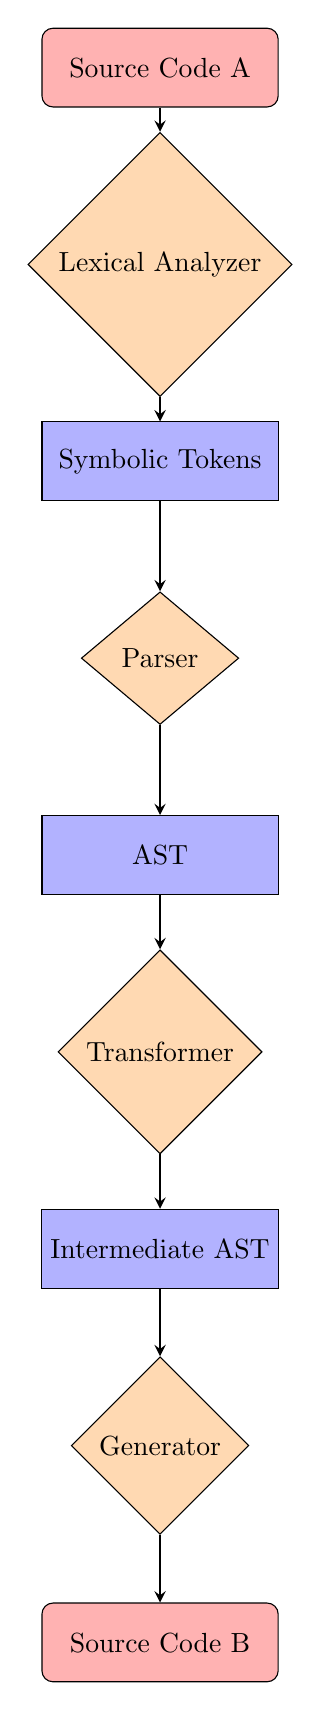
\begin{tikzpicture}[node distance=2.5cm]

    \node (sourcea) [startstop]                 {Source Code A};
    \node (lexer)   [process, below of=sourcea] {Lexical Analyzer};
    \node (tokens)  [io, below of=lexer]        {Symbolic Tokens};
    \node (parser)  [process, below of=tokens]  {Parser};
    \node (asta)    [io, below of=parser]       {AST};
    \node (trans)   [process, below of=asta]    {Transformer};
    \node (astb)    [io, below of=trans]        {Intermediate AST};
    \node (gen)     [process, below of=astb]    {Generator};
    \node (stop)    [startstop, below of=gen]   {Source Code B};

    \draw [arrow] (sourcea) -- (lexer);
    \draw [arrow] (lexer) -- (tokens);
    \draw [arrow] (tokens) -- (parser);
    \draw [arrow] (parser) -- (asta);
    \draw [arrow] (asta) -- (trans);
    \draw [arrow] (trans) -- (astb);
    \draw [arrow] (astb) -- (gen);
    \draw [arrow] (gen) -- (stop);

\end{tikzpicture}

\subsection{Abstracting Language Definitions}

To parse an input language, Glossa needs a description of the languages grammar, which is provided through a \textit{grammar file}.
Optional descriptions of AST transformations are provided through \textit{transformer files}.

To generate an output language from an AST, Glossa needs a set of \textit{constructor files}.

\subsection{Grammar Files}

Glossa's parse operation can be modeled as a function with the signature:

\begin{verbatim}
parse :: Tokens -> AST
\end{verbatim}

Where the body of the parse function looks like:

\lstset{language=Python}
\begin{lstlisting}
while not tokens.empty():
    identify_remaining(tokens)
\end{lstlisting}

Glossa will attempt to identify remaining tokens with any of the high-level statement types provided.
These statement types can use other grammar constructs as well

A single grammar files defines a potential identification of tokens, producing a tagged dictionary of symbols if the tokens are identified successfully:

The simplest non-trivial grammar file is likely the assignment statement:
\begin{verbatim}
assignment: `@lval identifier **` `@op '='` `@rval boolexpression | expression`
\end{verbatim}

In plain english this reads:
\textit{"Parse an identifier, and save it to the symbol dictionary as `lval`, then parse an equals operator, and save it to `op`, lastly, parse a boolean expression or normal expression and save it to `rval`"}

In general, a grammar element is defined like the following:

\begin{verbatim}
name: `first_element` `second_element`
\end{verbatim}

Where first\_element and second\_element are parsers of the form:

\begin{verbatim}
an optional "@name" tag, which saves the result of the parser to the symbol dictionary under "name"
Either:
- A subtype parser (i.e `'='`),
- A subtype-type parser (i.e. `identifier self`)
- A type parser (i.e. `identifier **`)
- A link to another grammar element (i.e. `value`)

So, the following are all examples of valid parsers:
`@val value`          // Link to value type, saved as "val"
`identifier self`     // Identifier "self", discarded
`@name identifier **` // Any identifier saved as "name"

However, these parsers can be prefixed with the following keywords to change their meaning:

!           : discard the parse result of this parser
anyOf a b   : parse either a or b, keeping the result of the first successful parser. 
    (alternatively written a | b) 
*/many      : parse the parser several times until it fails
many1       : parse the parser several times, requiring it to parse successfully at least once
optional    : make a parser optional
inOrder a b : run several parsers in order
sep a b     : parse bs seperated by as (i.e. sep , value) 

Some examples of more sophisticated parsers

`@statement import_from | main | ... ` 
`@val identifier ** | string | literal ** | 'None' | 'True' | 'False'`
`@val vector | functioncall | elementaccess | memberaccess | basevalue | parenexpr`
`@args optional sep ',' expression`
\end{verbatim}

So, fully formed grammar elements (for Python) look like:
\begin{verbatim}
main: 'if' '__name__' '==' `literal string` ':' `@body *statement` 'end'

function: 'def' `@identifier identifier **` '(' `@args optional sep ',' identifier **` ')' ':' `@body *statement` 'end' 

pass: 'pass'

return: 'return' `@expression expression`

assignment: `@lval identifier **` `@op '='` `@rval boolexpression | expression`

\end{verbatim}

\subsection{AST Transformations}

Transformations to the AST allow for an overall simpler compilation process, reducing the number of construction files required for an output language. Essentially, transformations change language-specific features into more generalized ones. AST transforms can also model code optimizations.

[Detail of how transformer files work]

\subsection{Constructors}

Constructor files describe how to build generalized syntax features. Mostly, they look like code in the output language, but with the elements replaced with tags from the symbol dictionary.
i.e. an assignment statement in c++
\lstset{language=c++}
\begin{lstlisting}
auto $lval$ $op$ $rval$
\end{lstlisting}
might become
\lstset{language=c++}
\begin{lstlisting}
auto x = 42
\end{lstlisting}
However, if we wish to reassign to a variable, the auto type declaration needs to be left off, so we might redefine the constructor file as:
\begin{verbatim}
branch defined lval 
$lval$ $op$ $rval$
elsebranch
auto $lval$ $op$ $rval$
end
\end{verbatim}
Where "defined lval" checks if lval is part of the namespace
How does lval get inserted into the namespace in the first place?
Constructor files must define which values will be put into the namespace, so our full constructor file would start with:
\begin{verbatim}
defines
lval
\end{verbatim}
Additionally, c++ has both header and source files in generation, but assignment statements look the same for each.
Our full constructor file looks like:

\begin{verbatim}
defines
lval

header
branch defined lval 
$lval$ $op$ $rval$
elsebranch
auto $lval$ $op$ $rval$
end

source
branch defined lval 
$lval$ $op$ $rval$
elsebranch
auto $lval$ $op$ $rval$
end
\end{verbatim}

Where "header" and "source" are defined in the special cpp/constructors/file file, which outlines which filetypes c++ will construct

% ==================================================
\section{Applications}
% ==================================================

Glossas core focus is on language design and creation. Creation of new languages and extension of existing ones should be very simple. 

\subsection{Glossa as a pre-processor}

Since Glossa can convert one language to another, it works as a pre-processor.
Glossa has the ability for languages to inherit from and extend other languages, so, for example, C++ might inherit from C, and then implement class statements that compile into C code.

\subsection{Language Creation, Design, and Modification}

In its ability to create new languages and extend existing ones, Glossa aims to help programming language research.
If syntax features can be quickly added or removed, programming languages will evolve more rapidly.
Rapid development of programming languages leads to better programming languages.

\subsection{Simple code porting}

Additionally, Glossa is able to port code. For example, Glossa can easily re-implement software like 2to3, which updates old python code.
For outdated projects, or projects written in too many languages, easy conversions between languages are extremely useful.

% ==================================================
\section{Results}
% ==================================================

% ==================================================
\section{Conclusion}
% ==================================================

% ==================================================
\section{Appendix}
% ==================================================

\newpage
\subsection{Original Python Code}

\lstset{language=Python}
\begin{lstlisting}
def sort(array):
    less    = []
    equal   = []
    greater = []

    if len(array) <= 1:
        return array
    else:
        pivot = array[0]
        for x in array:
            if x < pivot:
                less.append(x)
            if x == pivot:
                equal.append(x)
            if x > pivot:
                greater.append(x)
        return sort(less) + equal + sort(greater)

def main():
    l = sort([3, 2, 12, 9, 4, 68, 17, 1, 2, 3, 4, 5, 6, 12, 9  , 8, 7, 6,5, 4, 743])

if __name__ == "__main__":
    main()
\end{lstlisting}

\lstset{language=C}

\newpage
\subsection{Generated C++ Code (Glossa)}

\begin{lstlisting}
#include "../std/std.hpp"
template <typename T_array>
auto sort (T_array array)
{
    auto less = std::vector<Object>({});
    auto equal = std::vector<Object>({});
    auto greater = std::vector<Object>({});
    if (len(array) <= 1)
    {
        return array;
    }
    else
    {
        auto pivot = array[0];
        for (auto x : array)
        {
            if (x < pivot)
            {
                less.push_back(x);
            }
            if (x == pivot)
            {
                equal.push_back(x);
            }
            if (x > pivot)
            {
                greater.push_back(x);
            }
        };
        return sort(less) + equal + sort(greater);
    };
}
\end{lstlisting}

\newpage
\subsection{Generated C Code (Cython)}

Generated code for Cython is much more complex, as it integrates with the Python FFI

For example, this snippet declares an empty array

\begin{lstlisting}
  /* "main.py":6
 *     Sorts an array of comparable values
 *     """
 *     less    = []             # <<<<<<<<<<<<<<
 *     equal   = []
 *     greater = []
 */
  __pyx_t_1 = PyList_New(0); if (unlikely(!__pyx_t_1)) {__pyx_filename = __pyx_f[0]; __pyx_lineno = 6; __pyx_clineno = __LINE__; goto __pyx_L1_error;}
  __Pyx_GOTREF(__pyx_t_1);
  __pyx_v_less = ((PyObject*)__pyx_t_1);
  __pyx_t_1 = 0;
\end{lstlisting}

\newpage

\end{document}
